\documentclass[a4paper,11pt]{jsarticle}


% 数式
\usepackage{amsmath,amsfonts}
\usepackage{bm}
\usepackage{physics}
% 画像
\usepackage[dvipdfmx]{graphicx}
% ローマ数字
\usepackage{otf}
%単位
\usepackage{siunitx}
%表
\usepackage{multirow}
\usepackage{url}

\begin{document}

\title{物理学実験\ajRoman{2}レポート(パルス技術2Ab)}
\author{05-211525 齋藤駿一\\
共同実験者:菅原優生}
\date{\today}
\maketitle

\section{実験1}
まずパルス発生器で発生させたパルスをGATE\;\&\;Delay\;Generatorで整形し,可変減衰器で適切に減衰させ,その波形をオシロスコープで確認できるようにセットアップを行った.
オシロスコープに繋がる同軸ケーブルには,その特性インピーダンスに等しい\SI{50}{\ohm}の終端抵抗をつけた.

\subsection{課題1.1}
\subsubsection{手法と結果}
まずパルス発生器のパルスのレートを\SI{100}{\kHz}に設定した.
次にGATE\;\&\;Delay\;Generatorの遅延時間を0に,パルス幅を\SI{1}{\us}に設定した.
最後に可変減衰器で減衰度を調整し,オシロスコープ上でパルスの波高が$+$\SI{1.0}{V}となるようにした.
その結果図\ref{fig:pulserise}のような波形が得られた.

\begin{figure}[htbp]
  \centering
  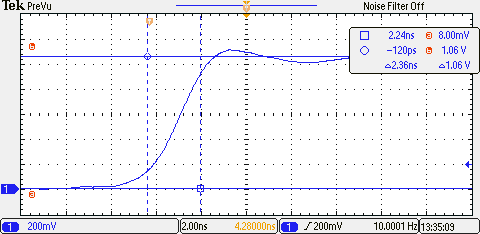
\includegraphics[width=10cm]{TEK00726.png}
  \caption{矩形波パルス(幅\SI{1}{\um},波高$+$\SI{1.0}{V})の立ち上がりの様子}
  \label{fig:pulserise}
\end{figure}

ここでは「パルスの高さ」を,パルスが安定して平坦になったところでの波高と定義する.
また「立ち上がり時間」を,波高がパルスの高さの10\%から90\%になるのにかかる時間と定義する.

まず得られたパルスの立ち上がり時間をディスプレイ上で測定した値から求める.
オシロスコープのカーソルを操作して,図\ref{fig:pulserise}に示したパルスは\SI{8.00}{\mV}から\SI{1.06}{V}に立ち上がっていることを確認した.
よって波高がパルスの高さの10\%に達したときの電位は約\SI{113}{\mV},90\%に達したときの電位は約\SI{955}{\mV}と計算できる.
ただしカーソルは離散的に動くので,正確にこれらの電位に達した時刻を測定することは難しかった.
そこでこれらに最も近い電位\SI{112}{\mV},\SI{952}{\mV}に達したときの時刻を確認したところ,それぞれ\SI{-360}{\ps},\SI{2.36}{\ns}であった.
よってパルスの立ち上がり時間はその差をとって約\SI{2.72}{\ns}と分かる.

\subsubsection{考察}
ディスプレイに表示される波形は,実際にはオシロスコープ自身の立ち上がり時間の寄与を受ける,
オシロスコープの周波数帯域$f_{\mathrm{osc}}=\SI{200}{\MHz}$から,オシロスコープによる立ち上がり時間は
\begin{equation}
  t_{\mathrm{osc}} = \frac{\SI{350}{\ns\per\MHz}}{f_{\mathrm{osc}}} = \SI{1.75}{\ns}
\end{equation}
となる.
これをもとに先ほど求めた立ち上がり時間$t_{\mathrm{disp}} = \SI{2.72}{\ns}$を補正すると,実際のパルスの立ち上がり時間は
\begin{equation}
  t_{\mathrm{pulse}} = \sqrt{t^2_{\mathrm{disp}} - t^2_{\mathrm{osc}}} = \SI{2.08}{\ns}
\end{equation}
と求まる.

\subsection{課題1.2}
課題1.1で用いたセットアップを次のように変更した.
まずオシロスコープのCH1に繋がる同軸ケーブルの終端抵抗を取り外し,代わりに\SI{1}{m}(メジャーを用いて長さを正確に測定した結果\SI{101.7}{\cm}と分かった.)の同軸ケーブルを取り付けた.
そしてケーブルの反対側をオシロスコープのCH2に接続し,そこに\SI{50}{\ohm}の終端抵抗を取り付けた.
またオシロスコープのディスプレイ上にCH2の信号が表示されるようにした.
その結果図\ref{fig:1m_cable}のように,CH1と似た波形がCH2で遅れて立ち上がることが分かった.
またCH1,CH2のそれぞれの波形で立ち上がった直後に電圧値が極大をとる時刻にカーソルを合わせ,その差を確認すると\SI{5.28}{\ns}と分かった.

次にCH1とCH2の間のケーブルの長さを\SI{5}{m}(メジャーを用いて長さを正確に測定した結果\SI{501.9}{\cm}と分かった.)に変更して同じ測定を行った.
その結果図\ref{fig:5m_cable}が得られ,立ち上がりの時刻の差は\SI{26.8}{\ns}と分かった.

これより同軸ケーブルを伝わるパルスの速度は
\begin{equation}
  v = \frac{\SI{501.9}{\cm} - \SI{101.7}{\cm}}{\SI{26.8}{\ns}- \SI{5.28}{\ns}} = \SI{18.6}{\cm\per\ns} = \SI{1.86e8}{m\per s}
\end{equation}
と求まる.
これは真空中の光速度の約62\%である.

\begin{figure}[htbp]
  \centering
  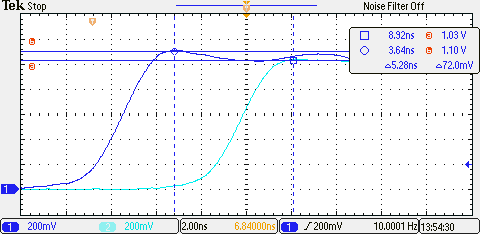
\includegraphics[width=10cm]{TEK00727.png}
  \caption{直接オシロスコープに入ったパルス(青色)と,そこからさらに長さ\SI{1}{m}の同軸ケーブルを通ってからオシロスコープに入ったパルス(水色)の波形}
  \label{fig:1m_cable}
\end{figure}

\begin{figure}[htbp]
  \centering
  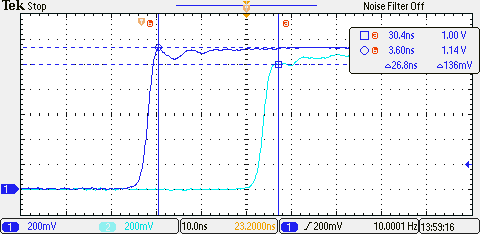
\includegraphics[width=10cm]{TEK00728.png}
  \caption{直接オシロスコープに入ったパルス(青色)と,そこからさらに長さ\SI{5}{m}の同軸ケーブルを通ってからオシロスコープに入ったパルス(水色)の波形}
  \label{fig:5m_cable}
\end{figure}

\subsection{課題1.3}
課題1.2のセットアップ(CH1とCH2の間のケーブルの長さを\SI{5}{m}としたもの)を引き続き用い,CH2に取り付けた終端抵抗を他のものに変えてオシロスコープの波形を観察した.

\subsubsection{終端抵抗を短絡させた場合($R=0$)}
終端抵抗を短絡させると図\ref{fig:R=0}のような波形が得られた.
この場合パルスがケーブル終端に達すると符号が逆転した反射波が生じる.
そのため速度$v$で進むパルスが長さ$L$のケーブルを往復するのにかかる時間$2L/v$だけ経過すると,ケーブル直前の位置で入力のパルスと反射したパルスが打ち消し合う.
その結果として,ケーブル直前では時刻0でパルスが立ち上がり,時刻$2L/v$でパルスが反射波に打ち消され,電圧値が0に戻ったと考える.

\begin{figure}[htbp]
  \centering
  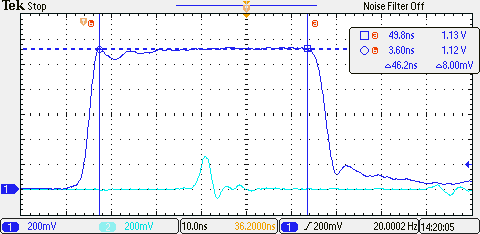
\includegraphics[width=10cm]{TEK00729.png}
  \caption{ケーブル終端を短絡させた場合の波形($R=0$).青色は\SI{5}{m}のケーブル直前の波形,水色はケーブル直後の波形.}
  \label{fig:R=0}
\end{figure}

\subsubsection{終端に(同軸ケーブルの特性インピーダンスとは異なる)有限の抵抗を繋いだ場合($R=\SI{83}{\ohm}, \SI{100}{\ohm}$)}
同軸ケーブルの特性インピーダンス(\SI{50}{\ohm})と異なる抵抗を終端に繋いだところ,$R=\SI{83}{\ohm}$では図\ref{fig:R=83},$R=\SI{100}{\ohm}$では図\ref{fig:R=100}のような波形が得られた.

まず同軸ケーブルの特性インピーダンスを$Z_0$,終端抵抗のインピーダンスを$Z_L$とおくと,終端での反射係数は
\begin{equation}
  r = \frac{Z_L - Z_0}{Z_L + Z_0}
\end{equation}
と与えられる.
今回の終端抵抗はいずれも$Z_0=\SI{50}{\ohm}$より大きいので,$r>0$,つまり反射波は同符号となる.
その結果として,ケーブル直前では時刻0でパルスが立ち上がり,時刻$2L/v$でパルスに反射波が加わってさらに電圧値が上昇したと考える.

今回は実験していないが,逆に$Z_0=\SI{50}{\ohm}$よりも小さい終端抵抗を繋げた場合,$r<0$となるので時刻$2L/v$で電圧値は下がると考える.

\begin{figure}[htbp]
  \centering
  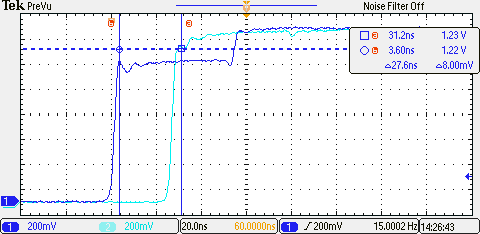
\includegraphics[width=10cm]{TEK00730.png}
  \caption{ケーブル終端に抵抗(\SI{83.37}{\ohm})を取り付けた場合の波形.青色は\SI{5}{m}のケーブル直前の波形,水色はケーブル直後の波形.}
  \label{fig:R=83}
\end{figure}

\begin{figure}[htbp]
  \centering
  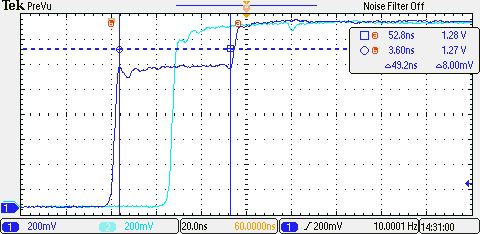
\includegraphics[width=10cm]{TEK00731.png}
  \caption{ケーブル終端に抵抗(\SI{100.24}{\ohm})を取り付けた場合の波形.青色は\SI{5}{m}のケーブル直前の波形,水色はケーブル直後の波形.}
  \label{fig:R=100}
\end{figure}

\subsubsection{ケーブル終端に何も取り付けなかった場合($R=\infty\,\si{\ohm}$)}
ケーブル終端に何も取り付けなかった場合,図\ref{fig:R=inf}のような波形が得られた.
ケーブル終端に何も取り付けない場合,ケーブル終端で同軸ケーブルの芯線と外部導線の間で電荷の移動がないので,入射波とまったく同じ反射波が生じる.
その結果として,ケーブル直前では時刻0にパルスが立ち上がり,時刻$2L/v$でパルスに反射波が加わって電圧値が2倍になったと考える.

\begin{figure}[htbp]
  \centering
  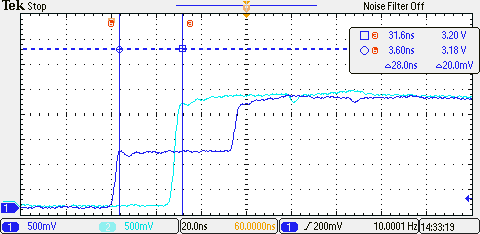
\includegraphics[width=10cm]{TEK00732.png}
  \caption{ケーブル終端に何も取り付けなかった場合の波形($\infty$\,\si{\ohm}).青色は\SI{5}{m}のケーブル直前の波形,水色はケーブル直後の波形.}
  \label{fig:R=inf}
\end{figure}

\subsubsection{ケーブル終端にコンデンサ,コイルを取り付けた場合}
ケーブル終端にコンデンサを取り付けた場合図\ref{fig:C=493},コイルを取り付けた場合図\ref{fig:L=0.39}のような波形が得られた.
これらについて取り付けた素子のインピーダンスから反射係数を求めることもできるが,ここではそれはせず定性的な考察を行う.
コンデンサは電流が流れ始めるときは抵抗が0のような振る舞いをし,定常状態では抵抗が$\infty$のような振る舞いをすることが知られている.
よって今回の場合の反射波も,最初は$R=0$のときと同じく入射波を打ち消すが,徐々に$R=\infty$のときのように入射波を2倍に増幅させるようになると考える.
その結果として,ケーブル直前では時刻0でパルスが立ち上がり,時刻$2L/v$で一度反射波により電圧値が0に近づくが,その後電圧値が上昇してもとのパルスの2倍の高さに近づいていくと考える.

一方コイルは電流が流れ始めるときは抵抗が$\infty$のような振る舞いをし,定常状態では抵抗が0のような振る舞いをすることが知られている.
その結果としてコンデンサのときとは逆に,時刻$2L/v$で反射波により電圧値が上昇するが,その後電圧値が下降しもとのパルスが打ち消されると考える.

\begin{figure}[htbp]
  \centering
  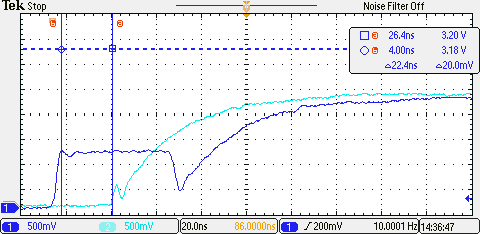
\includegraphics[width=10cm]{TEK00733.png}
  \caption{ケーブル終端にコンデンサ(\SI{492.9}{\pF})を取り付けた場合の波形.青色は\SI{5}{m}のケーブル直前の波形,水色はケーブル直後の波形.}
  \label{fig:C=493}
\end{figure}

\begin{figure}[htbp]
  \centering
  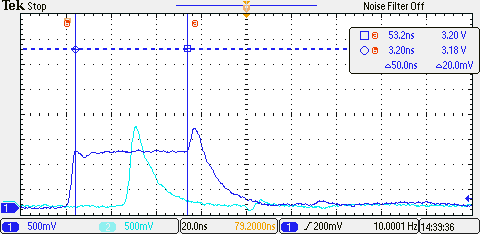
\includegraphics[width=10cm]{TEK00734.png}
  \caption{ケーブル終端にコイル(\SI{0.39}{\micro H})を取り付けた場合の波形.青色は\SI{5}{m}のケーブル直前の波形,水色はケーブル直後の波形.}
  \label{fig:L=0.39}
\end{figure}


\section{実験2}
プラスチックシンチレータ用光電子増倍管(PMT)信号A-GのうちAをオシロスコープのCH1に繋げた.
オシロスコープ側には\SI{50}{\ohm}の終端抵抗を取り付けた.
次に高圧電源の電圧出力を電圧分配器を通してそれぞれの光電子増倍管の$-$HVに印加した.
このとき徐々に電圧を上げ,最終的に\SI{-2000}{V}の電圧をかけた.

続いてNaIシンチレータ用光電子増倍管信号をオシロスコープのCH2に繋げた.
先ほどと同様ターミネートも行った.
その後この光電子増倍管に高圧電圧を印加した.
このとき\SI{10}{V}の出力設定つまみを回して徐々に電圧を上げ,\SI{+2000}{V}の電圧をかけた.

\subsection{課題2.1}
まずシンチレータ付近にCs線源を置きオシロスコープ上の波形を観察したところ,プラスチックシンチレータでは図\ref{fig:cs_pla},NaIシンチレータでは図\ref{fig:cs_nai}のような波形が得られた.

\begin{figure}[htbp]
  \centering
  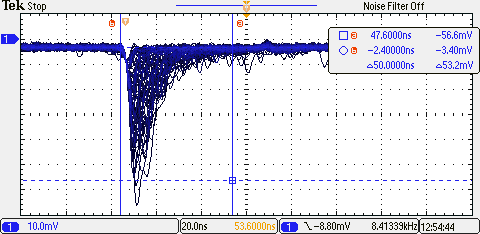
\includegraphics[width=10cm]{TEK00735.png}
  \caption{Cs線源近くのプラスチックシンチレータからの波形}
  \label{fig:cs_pla}
\end{figure}

\begin{figure}[htbp]
  \centering
  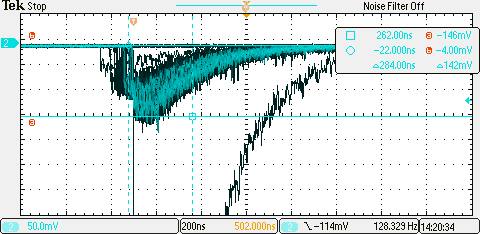
\includegraphics[width=10cm]{TEK00745.png}
  \caption{Cs線源近くのNaIシンチレータからの波形}
  \label{fig:cs_nai}
\end{figure}

次にNa線源を置いたところ,プラスチックシンチレータでは図\ref{fig:na_pla},NaIシンチレータでは図\ref{fig:na_nai}のような波形が得られた.

\begin{figure}[htbp]
  \centering
  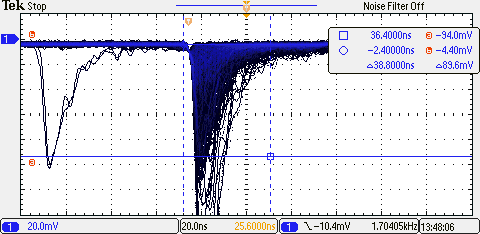
\includegraphics[width=10cm]{TEK00741.png}
  \caption{Na線源近くのプラスチックシンチレータからの波形}
  \label{fig:na_pla}
\end{figure}

\begin{figure}[htbp]
  \centering
  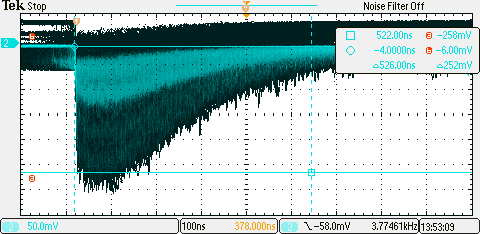
\includegraphics[width=10cm]{TEK00742.png}
  \caption{Na線源近くのNaIシンチレータからの波形}
  \label{fig:na_nai}
\end{figure}

\subsection{課題2.2}
課題2.1の結果をもとに,各シンチレータのエネルギー較正を行った.
まず課題2.1においてNaIシンチレータを通した波形では光電吸収ピークが見える.
そのためオシロスコープに表示された電圧はそのまま線源から放出された$\gamma$線のエネルギーに一致する.
一方プラスチックシンチレータを通した波形では光電吸収ピークは見えず,コンプトンエッジが見える.
そのためオシロスコープ上の電圧は線源から放出された$\gamma$線のエネルギーより小さなエネルギー値に対応する,

\begin{table}[htbp]
  \centering
  \caption{エネルギー較正に用いた値(1)}
  \label{tab:calib}  
  \begin{tabular}{c|cc|cc}
    &\multicolumn{2}{c|}{プラスチックシンチレータ}& \multicolumn{2}{c}{NaIシンチレータ}\\
    \hline
    線源 & エネルギー(MeV) & 電圧値(mV) & エネルギー(MeV) & 電圧値(mV)\\
    \hline\hline
    Cs & 0.478 & $50\pm 10$ & 0.662 & $130\pm 10$\\
    Na & 0.341 & $30\pm 7$ & 0.511 & $118\pm 6$ \\
    Na & 1.062 & $83\pm 7$ & 1.275 & $250\pm 10$ \\ 
    \hline
  \end{tabular}
\end{table}

各シンチレータに対して得られたデータをもとに較正を行った.
エネルギー$E$(MeV)の入力をプラスチックシンチレータに通すと,オシロスコープ上で電圧$V_{\mathrm{pla}}$(mV)の高さのパルスとして表示されるとする.
またNaIシンチレータに通すとそれが電圧$V_{\mathrm{NaI}}$(mV)の高さのパルスになるとする.
この各々に対して,実験結果から
\begin{equation}
  V_{i} = a_{i} E + b_{i} \qquad (i = \mathrm{pla}, \mathrm{NaI})
\end{equation}
という線形フィッティングを行った.
その結果
\begin{align}
  a_{\mathrm{pla}} &= 70 \pm 11 \\
  b_{\mathrm{pla}} &= 9 \pm 8 \\
  a_{\mathrm{NaI}} &= 174 \pm 19 \\
  b_{\mathrm{NaI}} &= 56 \pm 15
\end{align}
が得られ,図示するとプラスチックシンチレータの場合は図\ref{fig:calib_pla},NaIシンチレータの場合は図\ref{fig:calib_nai}のようになった.

\begin{figure}[htbp]
  \centering
  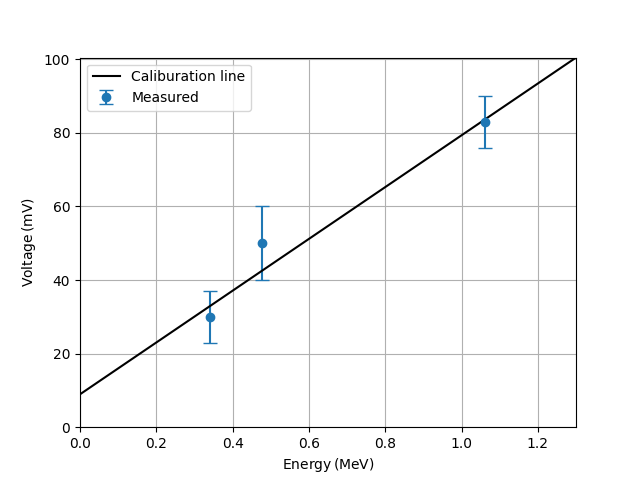
\includegraphics[width=10cm]{calib_pla.png}
  \caption{プラスチックシンチレータの較正直線:$V_{\mathrm{pla}}(\si{\mV}) = (70\pm 11) E(\si{\MeV}) + (9\pm 8)$}
  \label{fig:calib_pla}
\end{figure}

\begin{figure}[htbp]
  \centering
  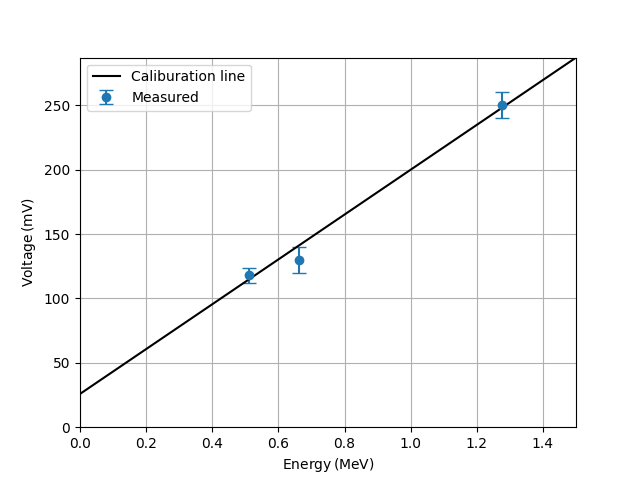
\includegraphics[width=10cm]{calib_nai.png}
  \caption{NaIシンチレータの較正直線:$V_{\mathrm{NaI}}(\si{\mV}) = (174\pm 19) E(\si{\MeV}) + (56\pm 15)$}
  \label{fig:calib_nai}
\end{figure}

\subsection{課題2.3}
$\mu$粒子がプラスチックシンチレータに入射したときエネルギー損失は\SI{2.01}{\MeV}であり,NaIシンチレータに入射したときエネルギー損失は\SI{6.08}{\MeV}である.
よって課題2.2で導いた較正直線から,$\mu$粒子はプラスチックシンチレータを通過すると\SI[separate-uncertainty]{150\pm 20}{\mV}のパルスを生み,NaIシンチレータを通過すると\SI[separate-uncertainty]{1080\pm 110}{\mV}のパルスを生むと計算できる.

\subsection{課題2.4}
課題2.1で扱った系から線源を取り除き,$\mu$粒子を測定した.
このとき課題2.3の計算結果が$\mu$粒子のエネルギーの平均値を与えることを参考にした.
ただし$\mu$粒子のエネルギー損失はLandau分布に従っており,平均値の半分程度のエネルギーを損失することもあるので,トリガーは求めた平均値の半分以下の位置にかけた.
その結果プラスチックシンチレータでは図\ref{fig:mu_pla}のような波形が,NaIシンチレータでは図\ref{fig:mu_nai}のような波形が見られた.
プラスチックシンチレータでは波形の現れる頻度は\SI[separate-uncertainty]{50\pm 20}{Hz}であり,理論値の\SI{20}{Hz}より高かった.
これはトリガレベルが約\SI{70}{\mV}だったため,$\mu$粒子以外の放射線による波形が混じったからと考える.
またNaIシンチレータでは波形の現れる頻度は1分に1回程度であり,これは理論値\SI{1.27}{\min^{-1}}と整合する.

\begin{figure}[htbp]
  \centering
  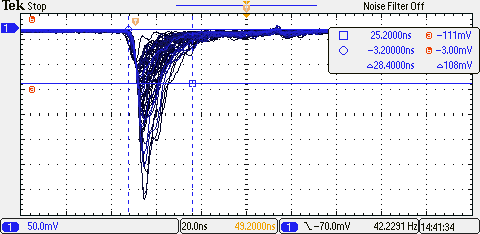
\includegraphics[width=10cm]{TEK00746.png}
  \caption{線源を離したときのプラスチックシンチレータからの波形.$\mu$粒子によるものと考える.}
  \label{fig:mu_pla}
\end{figure}


\begin{figure}[htbp]
  \centering
  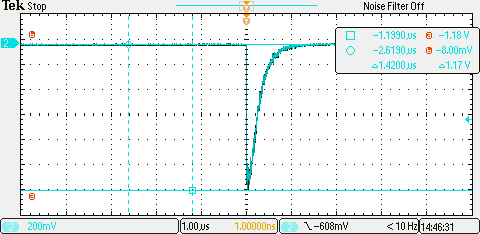
\includegraphics[width=10cm]{TEK00747.png}
  \caption{線源を離したときのNaIシンチレータからの波形.$\mu$粒子によるものと考える.}
  \label{fig:mu_nai}
\end{figure}

\section{課題3}
ここではディスクリミネータ回路,コインシデンス回路を用いて,宇宙線中での荷電粒子の強度とプラスチックシンチレータ中でのエネルギー損失を測定した.

\subsection{課題3.1}
\subsubsection{方法と結果}
\begin{figure}[htbp]
  \centering
  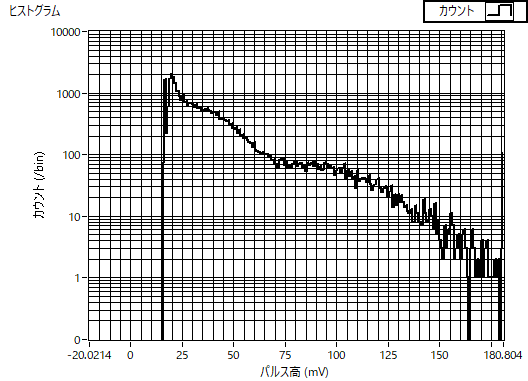
\includegraphics[width=10cm]{na_aself.png}
  \caption{Na線源を置いたときの信号のヒストグラム}
  \label{fig:na_aself}
\end{figure}

\begin{figure}[htbp]
  \centering
  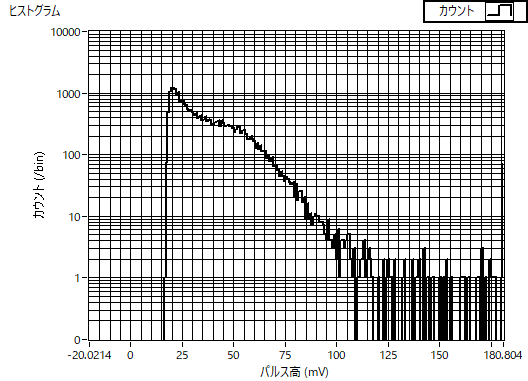
\includegraphics[width=10cm]{cs_aself.png}
  \caption{Cs線源を置いたときの信号のヒストグラム}
  \label{fig:cs_aself}
\end{figure}

\begin{table}[htbp]
  \centering
  \caption{エネルギー較正に用いた値(2)}
  \label{tab:calib2}  
  \begin{tabular}{c|cc}
    線源 & エネルギー(MeV) & 電圧値(mV) \\
    \hline\hline
    Cs & 0.478 & $50\pm 5$ \\
    Na & 0.341 & $40\pm 5$ \\
    Na & 1.062 & $110\pm 5$ \\ 
    \hline
  \end{tabular}
\end{table}

まずディスクリミネータのスレッショルド電圧を最低まで下げ,コインシデンス回路でシンチレータBに対応するものをOFFにした(以後この操作をシンチレータAのセルフトリガと呼ぶ).
つまりシンチレータAで起こったエネルギー損失を単純に記録した.
このときシンチレータ付近にNa線源を置いて数分待つと,エネルギー損失の実験結果(ヒストグラム)は図\ref{fig:na_aself}のようになった.
またCs線源に取り替えて同様の測定を行うと図\ref{fig:cs_aself}のようになった.

このヒストグラムにおいてコンプトンエッジは頻度が下がり始める部分にあると考え,コンプトンエッジの電圧値を表\ref{tab:calib2}のように求めた.
これをもとに較正を行うと
\begin{equation}
  V_{\mathrm{pla}}(\si{\mV}) = (99\pm 5) E(\si{\MeV}) + (5\pm 3)
\end{equation}
と求まった(図\ref{fig:calib2}).
以降では係数の誤差を切り捨てた式を較正に用い,$E$の比例係数の誤差の割合がおよそ$1/20$であることから誤差を見積もり,それをもとに有効数字を決めた.

\begin{figure}[htbp]
  \centering
  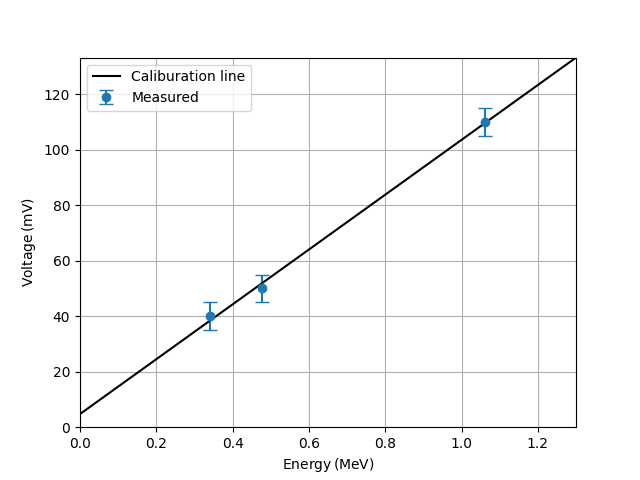
\includegraphics[width=10cm]{calib2.png}
  \caption{ヒストグラムを参照したエネルギー較正}
  \label{fig:calib2}
\end{figure}

次に線源を取り除き,宇宙線のエネルギー損失を測定した.
まず先ほどと同じくスレッショルド電圧を最低にし,Aのセルフトリガを行って測定すると,図\ref{fig:cosmray_low_aself}のようになった.
次にコインシデンス回路でシンチレータBに対応するものをONにして測定すると,図\ref{fig:cosmray_low_coin}のようになった.

前者は単にシンチレータAで起こったエネルギー損失の分布だが,後者はそのうちシンチレータA,Bで同時に起こったエネルギー損失を取り出した分布である.
$\mu$粒子が入射するとシンチレータA,Bで同時にエネルギー損失が起こるので,得られた二つの図を比較することで$\mu$粒子のエネルギー損失に対応する電圧が読み取れる.
この読み取りをもとにスレッショルド電圧を\SI{110}{\mV}に上げ,コインシデンス条件の下で測定を行うと図\ref{fig:cosmray_110mV_coin}のようになった.

\begin{figure}[htbp]
  \centering
  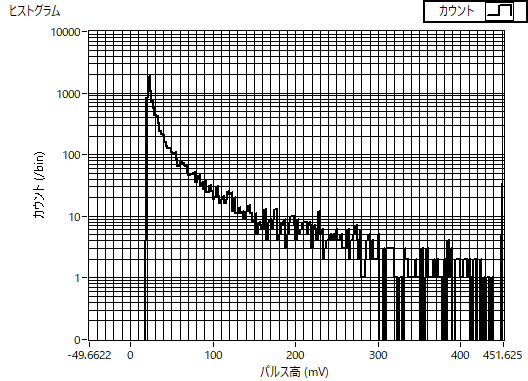
\includegraphics[width=10cm]{cosmray_low_aself.png}
  \caption{宇宙線のエネルギー損失を示すヒストグラム.シンチレータAのセルフトリガをかけて測定した.}
  \label{fig:cosmray_low_aself}
\end{figure}

\begin{figure}[htbp]
  \centering
  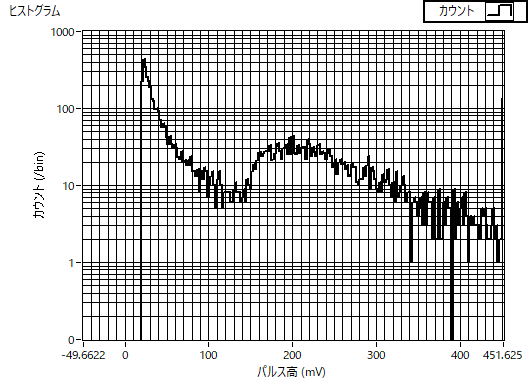
\includegraphics[width=10cm]{cosmray_low_coin.png}
  \caption{宇宙線のエネルギー損失を示すヒストグラム.コインシデンス条件を課して測定した.}
  \label{fig:cosmray_low_coin}
\end{figure}

\begin{figure}[htbp]
  \centering
  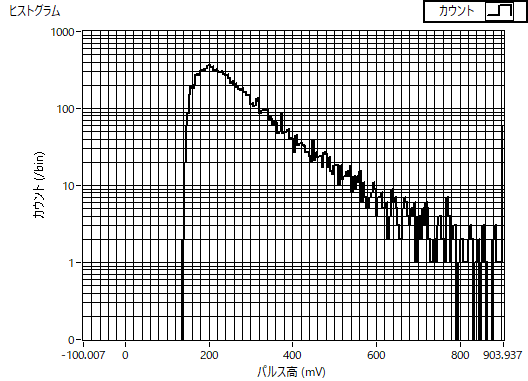
\includegraphics[width=10cm]{cosmray_110mV_coin.png}
  \caption{宇宙線のエネルギー損失を示すヒストグラム.スレッショルド電圧を\SI{110}{\mV}とし,コインシデンスを課した.}
  \label{fig:cosmray_110mV_coin}
\end{figure}

エネルギー損失の結果から,最頻値は\SI{2.0}{\MeV},平均値は\SI{2.6}{\MeV}と求まった.
この平均値はBethe-Blochの計算から導かれる\SI{2.01}{\MeV}よりも大きな値である.

\subsubsection{考察}
次にこの結果を考察する.
まず平均値が最頻値より大きいことから,エネルギー損失の分布は高エネルギー側に偏っているといえる.
これはエネルギー損失がLandau分布に従っており,高エネルギー側の裾野が広いためと考える.

一方で平均値がBethe-Blochの計算からずれた原因を考察する.
まず較正直線の誤差を考えると,較正直線の傾きに5\%の誤差があることから,それをもとに求めた平均値\SI{2.6}{\MeV}には\SI{0.1}{\MeV}の誤差がある.
これはBethe-Blochの計算からのずれよりも小さく,このずれの説明にはならない.
また今回の実験結果では平均値\SI{2.6}{\MeV}よりも最頻値\SI{2.0}{\MeV}の方がBethe-Blochの計算\SI{2.01}{\MeV}に近い.
先ほどと同様に誤差を考えると最頻値の誤差も\SI{0.1}{\MeV}となるので,最頻値はBethe-Blochの計算と一致するといえる.
しかし結局平均値とBethe-Blochの計算の差異は説明できなかった.

\subsection{課題3.2}
\subsubsection{測定結果}
また課題3.1で行った宇宙線のエネルギー損失の測定と同時に,各シンチレータに繋がったディスクリミネータ回路とコインシデンス回路から発せられたパルスの総数をカウントした.
その結果\SI{1434.4}{s}の間にシンチレータAに繋がったディスクリミネータ回路から24,970回,シンチレータBに繋がったディスクリミネータ回路から17,935,055回,コインシデンス回路から14,531回パルスが出たことが分かった.
またシンチレータA,Bのジオメトリーも測定した.
その結果シンチレータは一辺$L=\SI{35.5}{\cm}$の正方形で,シンチレータA,B間の距離は$d=\SI{8.0}{\cm}$と分かった.

\subsubsection{宇宙線のフラックスと計測率の関係}
これをもとに宇宙線のフラックスを求めた.
下側のシンチレータ上に点Pおよびそのまわりの微小面積$dS$をとり,上側のシンチレータ上に点P'およびそのまわりの微小面積$dS'$をとる.
このとき単位時間当たりに$dS'$から$dS$へと貫いていく宇宙線の総数を求める.
シンチレータに垂直な上向きの方向に$z$軸をとり,直線PP'と$z$軸のなす角を$\theta$とする.
まず点Pと点P'の間の距離を$r$とすると,点Pから$dS'$を見こむ立体角は$dS'\cos{\theta}/r^2$である.
よって宇宙線のフラックスを$I$とおくと,単位時間当たりに$dS'$を通過する宇宙線の総数は$IdS'\cos{\theta}/r^2$となる.
一方でこの宇宙線が$dS$に入射するとき,宇宙線は$dS$を宇宙線の入射方向に傾けた微小面積$dS\cos{\theta}$を通過する.
よって結局$dS'$を経由して$dS$へ単位時間当たりに到達する宇宙線の総数$dN/dt$は
\begin{equation}
  \frac{dN}{dt} = IdS'\frac{\cos{\theta}}{r^2} dS\cos{\theta} = \frac{I\cos^2{\theta}}{r^2}dSdS'
\end{equation}
となる.
よってある計測時間$t$の間に上側のシンチレータを経由して下側のシンチレータに到達する宇宙線の総数$N$は
\begin{equation}
  \frac{N}{t} = \iint \frac{I\cos^2{\theta}}{r^2} dSdS' 
  \label{cosm}
\end{equation}
と計算できる.
ただし積分は上下のシンチレータの全域にわたって行う.
また上下のシンチレータにそれぞれ$(x_1,y_1),(x_2,y_2)$の座標を入れると,シンチレータの間隔を$d$として
\begin{equation}
  \cos{\theta} = \frac{d}{\sqrt{(x_1 - x_2)^2 + (y_1 - y_2)^2 + d^2}}
\end{equation}
および
\begin{equation}
  r = \sqrt{(x_1 - x_2)^2 + (y_1 - y_2)^2 + d^2}
\end{equation}
がいえる.
よって式\eqref{cosm}は
\begin{equation}
  \frac{N}{t} = \iiiint \frac{Id^2}{\left((x_1 - x_2)^2 + (y_1 - y_2)^2 + d^2 \right)^2}dx_1dy_1dx_2dy_2
  \label{cosm2}
\end{equation}
となる.

\subsubsection{宇宙線のフラックスが方向によらない場合の考察}
まず宇宙線のフラックスが方向によらないと仮定する.
このとき式\eqref{cosm2}より,コインシデンス回路から出たパルスの総数$N$,計測時間$t$,宇宙線のフラックス$I=I_0$の間に
\begin{equation}
  \frac{N}{t} = I_0 \iiiint \frac{d^2}{\left((x_1 - x_2)^2 + (y_1 - y_2)^2 + d^2 \right)^2} dx_1dy_1dx_2dy_2
  \label{flux_const}
\end{equation}
が成り立つ.
ただし積分は$0\le x_i, y_i \le \SI{35.5}{\cm}\,(i=1,2)$の区間でとる.
実験で求めた値を代入し積分を刻み幅\SI{0.1}{\cm}で数値計算すると,宇宙線のフラックス$I_0$は\SI{3.9e-3}{\per\steradian\per\cm^2\per\s}と求まった.

\subsection{課題3.3}
次に宇宙線のフラックスが$I=I'_0\cos^2{\theta}$の形で与えられると考える.
このとき式\eqref{flux_const}に代わって
\begin{equation}
  \frac{N}{t} = I_0 \iiiint \frac{d^4}{\left((x_1 - x_2)^2 + (y_1 - y_2)^2 + d^2 \right)^{3}} dx_1dy_1dx_2dy_2
\end{equation}
が成り立つ.
課題3.2と同様に積分を刻み幅\SI{0.1}{\cm}で数値計算すると,宇宙線のフラックス$I'_0$は\SI{6.5e-3}{\per\steradian\per\cm^2\per\s}と求まった.

参考文献\cite{cosmray}によれば地表において垂直方向から来る運動量\SI{1}{\GeV \per c}以上の$\mu$粒子のフラックスは約\SI{7e-3}{\per\steradian\per\cm^2\per\s}である.
課題3.2で計算した値よりもここで計算した値の方がこの文献値に近い.
よって実際には$\mu$粒子のフラックスは$I=I'_0\cos^2{\theta}$の形で与えられると考えられる.

\subsection{課題3.4}
これまではコインシデンス回路からパルスが出力された場合シンチレータA,Bを同時にある粒子が通過したと見なした.
ところが偶然二つの粒子が別々にシンチレータA,Bに入射したことで生じた無関係なパルスによってコインシデンス回路からパルスが出力されることもあり得る.
そこでここではその確率を見積もった.

まず\SI{1434.4}{s}の間にシンチレータAに繋がったディスクリミネータ回路から24,970回パルスの出力があった.
またパルス幅を測定すると\SI{60.0}{\ns}だった.
よって計測時間全体においてシンチレータA由来のパルスが出力されている時間の割合は
\begin{equation}
  p_1 = \frac{24,970\times\SI{60.0}{\ns}}{\SI{1434.4}{s}} = 1.04\times 10^{-6}
\end{equation}
と求まる.
一方で同じ計測時間でシンチレータBに繋がったディスクリミネータ回路から17,935,055回パルスの出力があり,そのパルス幅は\SI{59.2}{\ns}であった.
よって計測時間全体においてシンチレータB由来のパルスが出力されている時間の割合は
\begin{equation}
  p_2 = \frac{17,935,055\times\SI{59.2}{\ns}}{\SI{1434.4}{s}} = 7.40\times 10^{-4}
\end{equation}
と求まる.
したがって偶然二つのパルスが重なる確率は
\begin{equation}
  p_1 p_2 = 1.04\times 10^{-6} \times 7.40 \times 10^{-4} = 7.73 \times 10^{-10}
\end{equation}
と求まる.
これは非常に小さい確率なので,コインシデンス回路からパルスが発生した場合には,それは同一の粒子によるものと考えて問題ない.

\section{実験4}
\subsection{課題4.1}
ここでは配布されたデータをもとに$\mu$粒子の寿命を見積もった.

まずデータを得るための測定方法を述べる.
この測定ではシンチレータA,B,C,D,E,F,Gを用いる.
シンチレータはこの順に上から並んでおり,シンチレータD,Eは他のシンチレータに比べて分厚い一つのシンチレータに繋がっている.
そのため$\mu$粒子はまずシンチレータA,B,Cを通過し,その後シンチレータD,Eで崩壊し,電子または陽電子を放出する.
その結果シンチレータD,Eからは$\mu$粒子の入射時と崩壊時の2回信号が生まれる.
以降は入射時の信号をstart信号と呼び崩壊時の信号をstop信号と呼ぶ.
まずD,Eから発された信号を$\mu$粒子によるものに限定するため,シンチレータA~Eで信号が生まれF,Gで信号が生まれないような信号だけを抽出するようなコインシデンス回路を入れる.
またstart信号に対応するstop信号が入力されない場合に備えて,start信号の入力から\SI{18}{\us}後にstop信号を生成して入力する.
こうして得たstart信号とstop信号をポケオシの別々のチャンネルに入力し,その時間差を測定する.

ここではこのような実験により得られたデータを統計的に処理した.
まず$\mu$粒子は確率的に崩壊するので,あるパラメータ$\lambda$を用いて粒子数$N$は
\begin{equation}
  -\frac{dN}{dt} = \lambda N
\end{equation}
に従って指数的に減少すると考える.
つまり$\mu$粒子の平均寿命を$\tau$として
\begin{equation}
  N(t) = N_0 \exp\left(-\frac{t}{\tau}\right)
\end{equation}
と考える.
この仮説が正しいかを以降の統計的な解析によって確かめる.

\subsubsection{ヒストグラムを用いた解析}

\begin{figure}[htbp]
  \centering
  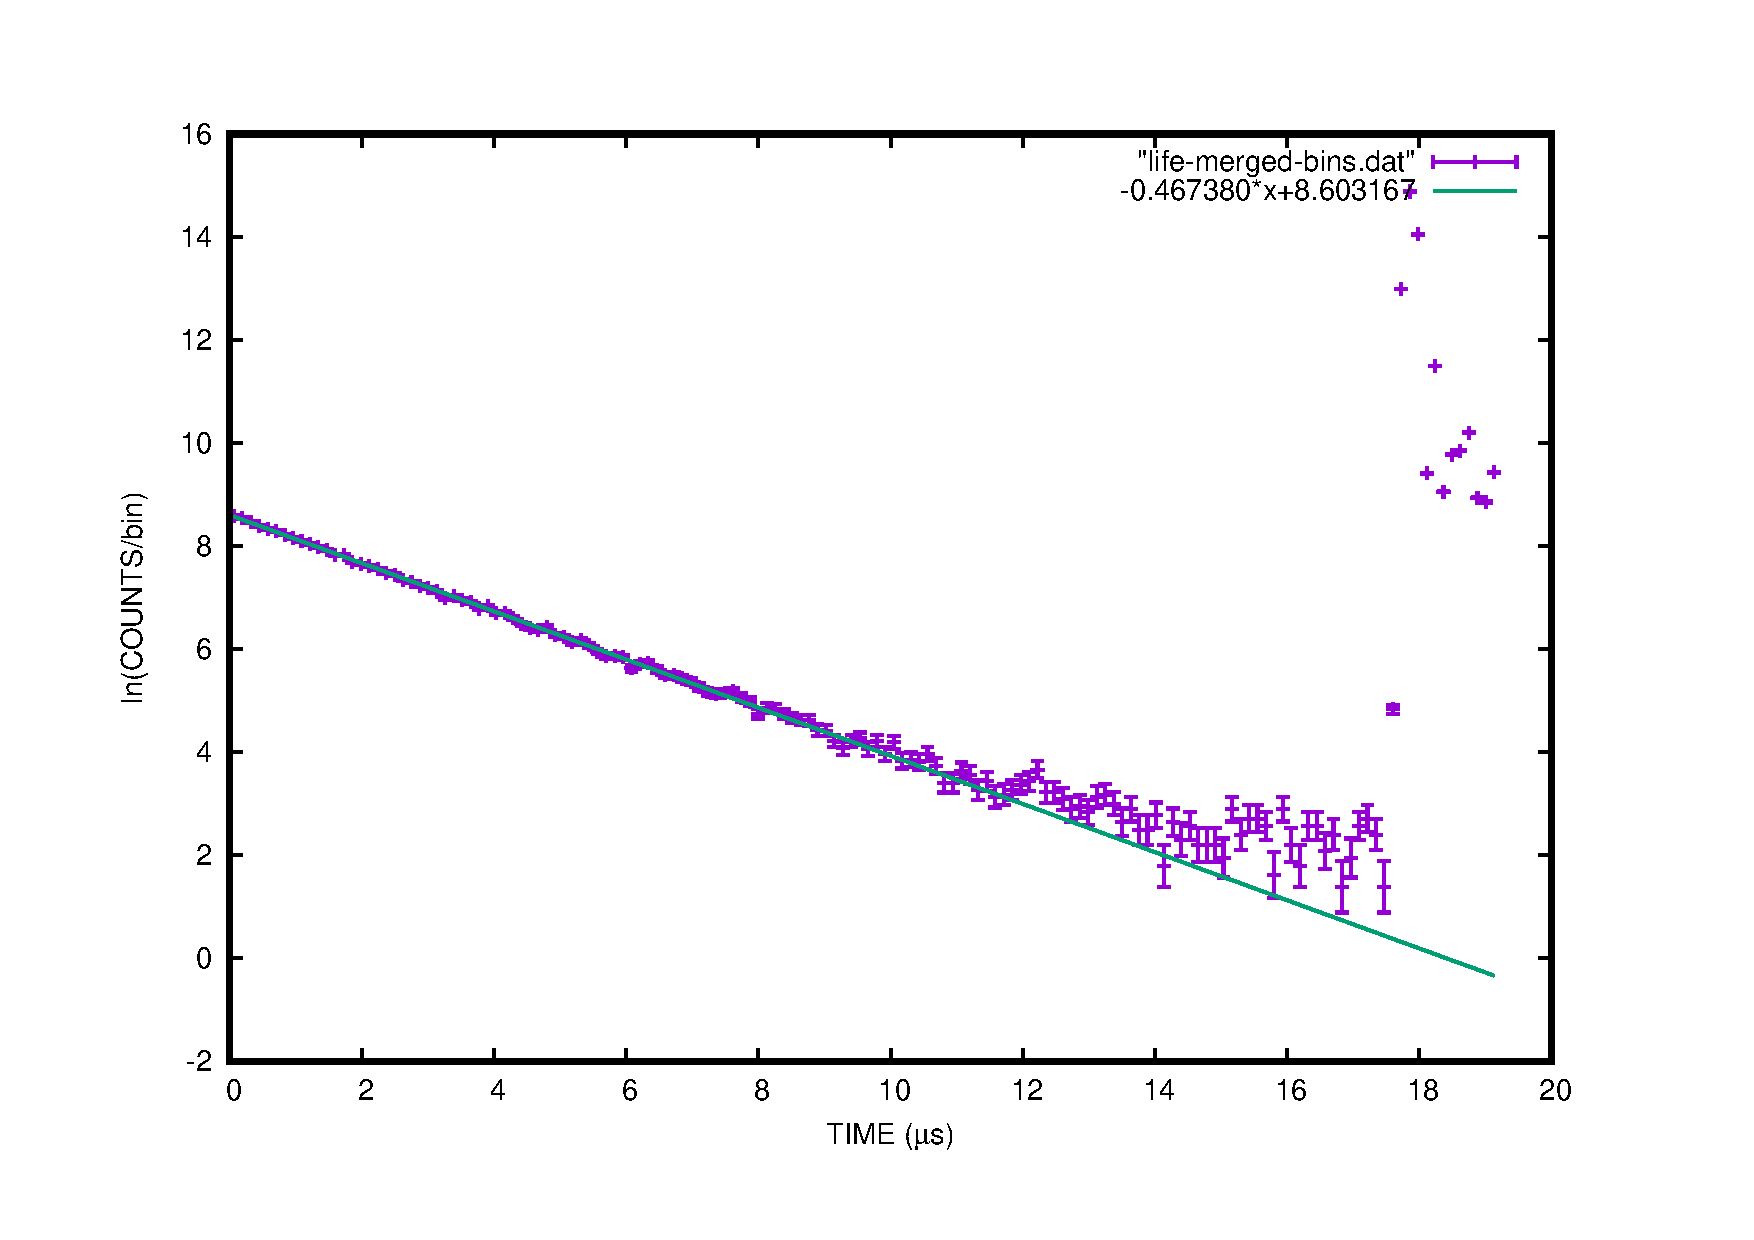
\includegraphics[width=13cm]{life.pdf}
  \caption{$\mu$粒子の入射から崩壊までの時間のヒストグラム(紫)とフィッティング(緑).フィッティングはガウス分布への近似が成り立つと考える範囲(粒子数30個以上)に限り,\SI{18}{\us}の信号付近は除いて行った.その結果$\tau = \SI[separate-uncertainty]{2.140\pm 0.008}{\us}$および$\chi^2/n=1.07$を得た.}
  \label{fig:life}
\end{figure}

まずデータを計測時間(start信号からstop信号までの時間)によって256個に分割してヒストグラムを作成した.
ヒストグラムのあるビン$j$に注目するとその個数は真の値$\mu_j$に対して統計的なばらつきでずれている.
そのばらつきはポアソン分布に従うと考える.
$\mu_j \gg 10$のときポアソン分布はガウス分布に近似できるので,このとき尤度$\mathcal{L}$は
\begin{equation}
  \mathcal{L} = \prod_j \frac{1}{\sqrt{2\pi \mu_j}}\exp\left( - \frac{(N_j-\mu_j)^2}{2\mu_j}\right)
\end{equation}
となる.

この確率を最大化するような$\mu_j$を考える(最尤法).
先ほどの仮説により$\mu_j=N_0\exp(-t/\tau)$なので,$\mu_j \approx N_j$および$\Delta N_j = \sqrt{N_j}$を用いると
\begin{equation}
  \chi^2 = \sum_j \frac{(N_j - N_0\exp(-t_j/\tau))^2}{\Delta N_j^2} 
\end{equation}
を最小化すれば良いことが分かる.
ここで変数変換$y_j = \ln{N_j}$を施すと,誤差の伝播則から$\Delta y_j = 1/\sqrt{N_j}$となることに注意して
\begin{equation}
  \chi^2 \approx \sum_j \frac{(y_j - \ln{N_0} + t/\tau)}{\Delta y_j^2}
\end{equation}
がいえる.
そこでこれを最小化するように関数
\begin{equation}
  f(t) = \alpha_0 + \alpha_1 t := \ln{N_0} - t/\tau
\end{equation}
を定めて平均寿命$\tau$を算出した.
またフィッティングの誤差$\Delta\alpha_0, \Delta\alpha_1$から$\tau$の誤差
\begin{equation}
  \Delta\tau = \frac{\Delta \alpha_1}{\alpha_1^2}
\end{equation}
も計算した.
そしてこのフィッティングをもとに$\chi^2$の最小値を計算した.
フィッティングに用いた点の数からパラメータの数2を引いた自由度$n$とこの$\chi^2$を比較して$\chi^2/n$を計算し,この値から仮説の信頼水準を求めた.

まずフィッティングの結果
\begin{equation}
  f(t) = (8.603\pm 0.005) + (-0.4674\pm 0.0016)t
\end{equation}
と分かった.
ただしガウス分布への近似が成り立つように,今回はフィッティングを$N_j \ge 30$のデータに限って行った.
また時間\SI{17}{\us}より先のデータを無視することで,\SI{18}{\us}付近の信号がフィッティングに寄与しないようにした.
このフィッティング結果より$\mu$粒子の寿命は$\tau = \SI[separate-uncertainty]{2.140\pm 0.008}{\us}$と計算できる.
またこのフィッティングをもとにカイ二乗検定を行うと$\chi^2=91.7$となり,自由度が$n=86$であることから
\begin{equation}
  \frac{\chi^2}{n} = 1.07
\end{equation}
となる.
これより信頼水準は約30\%と見積もれる\footnote{信頼水準の見積もりはテキストp.43の図38を参考にした.}.
よって$\mu$粒子の崩壊はポアソン分布で概ね良く近似できると考える.


\subsubsection{ヒストグラムを用いない解析}

次にヒストグラムを用いない別の方法で$\mu$粒子の寿命を推定した.
まずデータで得られた計測時間の測定値$t_k$は仮説より指数関数$\exp(-t/\tau)$に従うと考える.
よって尤度は
\begin{equation}
  \mathcal{L} = \prod_k \frac{1}{\tau} \exp\left(-\frac{t_k}{\tau}\right)
\end{equation}
と求まる.
これを最大化することは$\ln{\mathcal{L}}$を最大化することと等価である.
最大化が達成されたとき
\begin{equation}
  \pdv{\mathcal{L}}{\tau} = \sum_k\qty(-\frac{1}{\tau} + \frac{t_k}{\tau^2}) = 0
\end{equation}
より,イベント数を$n$とすると
\begin{equation}
  \tau = \frac{1}{n} \sum_k t_k
\end{equation}
がいえる.
つまり$\tau$の最良推定値はデータの平均である.
またその誤差$\Delta \tau$は$\ln{\mathcal{L}}$の尖り具合として
\begin{equation}
  \Delta \tau = \sqrt{\qty(-\left.\frac{\partial^{2} \mathcal{L}
  }{\partial \tau'^2}\right|_{\tau'=\tau})^{-1}} = \frac{\tau}{\sqrt{n}}
\end{equation}
と求まる.
以上の解析を計測時間\SI{17}{\us}以下のデータに対して行ったところ$\tau = \SI[separate-uncertainty]{2.171\pm 0.007}{\us}$と分かった.

\begin{figure}[htbp]
  \centering
  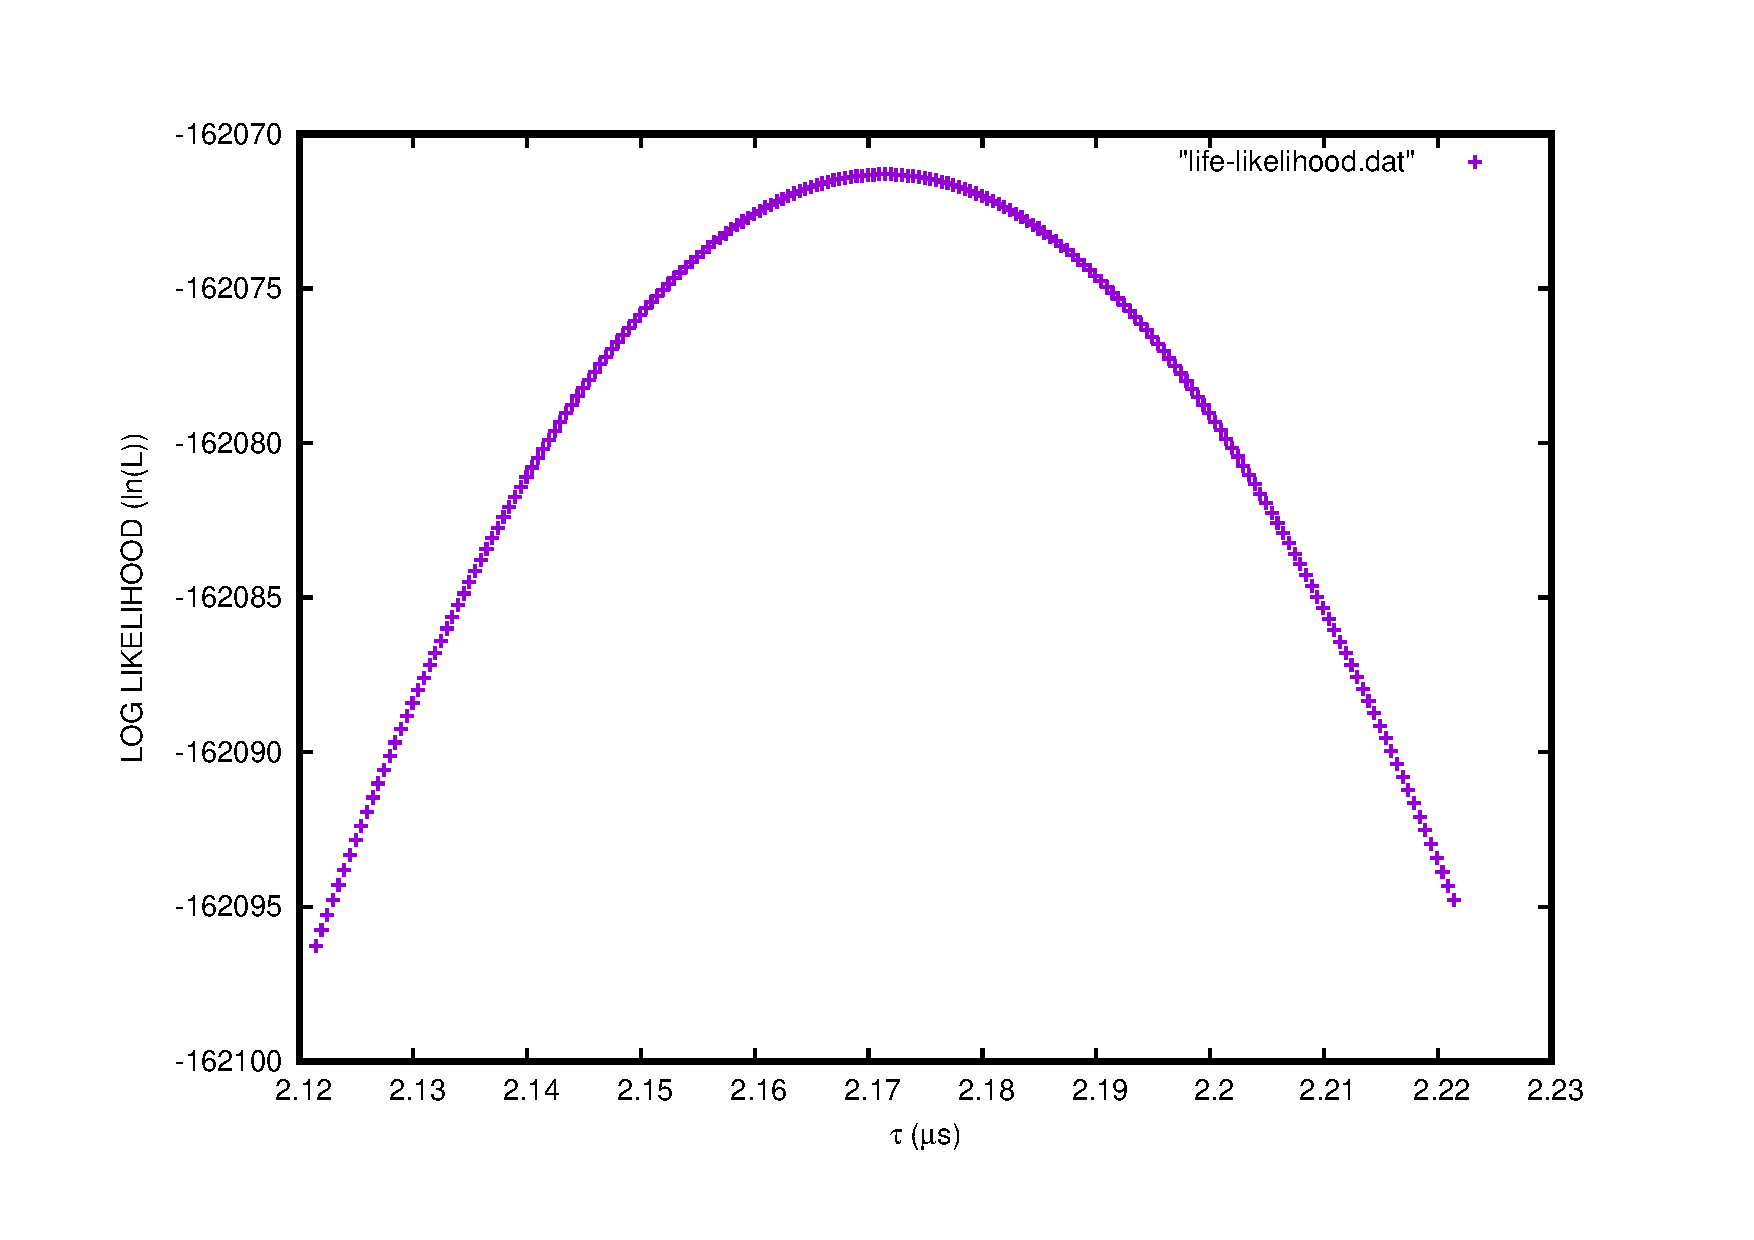
\includegraphics[width=13cm]{likelihood.pdf}
  \caption{$\mu$粒子の寿命の推定値$\tau$を変化させたときの尤度の対数$\ln{\mathcal{L}}$の変化.尤度が最大値をとる$\tau$を最良推定値として,$\ln{\mathcal{L}}$が0.5だけ下がった地点までを誤差とした.その結果$\tau=\SI[separate-uncertainty]{2.171\pm 0.007}{\us}$を得た.}
  \label{fig:likelihood}
\end{figure}

さらに別の方法で$\tau$を見積もる.
推定値$\tau$を変化させたときの尤度$\mathcal{L}$の対数は図\ref{fig:likelihood}のようになった.
そこでこのプロットの最大値における$\tau$を寿命の推定値と考える.
またこれと$\ln(\mathcal{L})$が最大値から0.5だけ下がった地点に最も近いプロットでの$\tau$までの差を$\tau$の誤差と考える.
このようにして求めた寿命は$\tau=\SI[separate-uncertainty]{2.171\pm 0.007}{\us}$となった.
これは先ほどの解析から求めた結果と完全に一致する.

\subsubsection{解析結果の考察}
まとめると,$\mu$粒子の寿命はヒストグラムを用いた解析では$\tau = \SI[separate-uncertainty]{2.140\pm 0.008}{\us}$,ヒストグラムを用いない解析では$\tau=\SI[separate-uncertainty]{2.171\pm 0.007}{\us}$と求まった.
一方で理科年表によれば電子や陽電子を出して崩壊する$\mu$粒子の寿命は\SI[separate-uncertainty]{2.19698\pm 0.00002}{\us}であり,今回の推定値はこれよりも有意に小さい.
これは崩壊して電子を放出する$\mu^{-}$がプラスチックシンチレータを構成する炭素によって原子核捕獲されるからと考える.
$\mu^{-}$粒子は原子核捕獲されると
\begin{equation}
  \mu^{-} + p \to \nu_{\mu} + n
\end{equation}
という反応を起こし,電子も陽電子も生じさせずに消失する.
そのため電子・陽電子の放出を伴う崩壊だけを考えたときの寿命\SI[separate-uncertainty]{2.19698\pm 0.00002}{\us}と比べて,今回の実験で得られる寿命は小さく見積もられることになる.

\begin{thebibliography}{99}
  \bibitem{text}
    「物理学実験\ajRoman{2}」解説書「パルス技術」2021年度

  \bibitem{cosmray}
    Partical Data Group, Review of Partical Physics, 30.Cosmic rays 
  
  \bibitem{nenpyo}
    国立天文台編「理科年表2019」

  \bibitem{tukuba}
    筑波大学素粒子実験室「$\mu$粒子寿命データの解析」\\
    \url{http://hep-www.px.tsukuba.ac.jp/~doraemon/class/exp3/Jikken3Day5.pdf}

\end{thebibliography}

\end{document}


\end{document}